\documentclass[a4,12pt,oneside,openany]{memoir}

\usepackage[utf8x]{inputenc}
\setlength{\parskip}{1em}

\usepackage{url}
\usepackage{amssymb,amsmath,amsthm,amsfonts}
\usepackage{mathtools}
\usepackage{overpic}
\usepackage{enumerate}
\usepackage{enumitem}
\usepackage{cleveref}
\usepackage{mathrsfs}
\usepackage[chapter]{algorithm}
\usepackage{algpseudocode}
\usepackage[top=1in, right=1in, left=1in, bottom=1in]{geometry}
\usepackage{tikz}
\usetikzlibrary{decorations.pathmorphing,arrows.meta}

\newcommand{\mX}{\mathcal{X}}
\newcommand{\mY}{\mathcal{Y}}
\newcommand{\mU}{\mathcal{U}}
\newcommand{\mV}{\mathcal{V}}
\newcommand{\mF}{\mathcal{F}}
\newcommand{\mG}{\mathcal{G}}
\newcommand{\mO}{\mathcal{O}}
\newcommand{\W}{\mathcal{W}}
\newcommand{\mH}{\mathcal{H}}
\newcommand{\mN}{\mathcal{N}}

\newcommand{\E}{\mathbb{E}}
\newcommand{\R}{\mathbb{R}}
\newcommand{\N}{\mathbb{N}}
\newcommand{\C}{\mathbb{C}}
\newcommand{\Z}{\mathbb{Z}}
\newcommand{\FFT}{{\rm FFT}}
\newcommand{\iFFT}{{\rm iFFT}}

\newcommand{\mcl}[1]{\mathcal{#1}}
\newcommand{\mbf}[1]{\mathbf{#1}}

\newcommand{\fb}{\mbf{f}}
\newcommand{\cb}{\mbf{c}}
\newcommand{\gb}{\mbf{g}}
\newcommand{\qb}{\mbf{q}}
\newcommand{\rb}{\mbf{r}}
\newcommand{\xb}{\mbf{x}}
\newcommand{\yb}{\mbf{y}}
\newcommand{\zb}{\mbf{z}}
\newcommand{\wb}{\mbf{w}}
\newcommand{\ub}{\mbf{u}}
\newcommand{\vb}{\mbf{v}}
\newcommand{\eb}{\mbf{e}}

\renewcommand{\bf}{\bfseries}
\renewcommand{\it}{\itshape}



%\newcommand{\cal}[1]{\mathcal{#1}}

\renewcommand{\hat}{\widehat}
\renewcommand{\tilde}{\widetilde}

\newcommand{\Span}{\mathrm{span}}

\DeclareMathOperator*{\argmax}{arg\,max}
\DeclareMathOperator*{\argmin}{arg\,min}

\usepackage[square,numbers,sectionbib]{natbib}
\usepackage{chapterbib}

\AtBeginDocument{\renewcommand{\bibsection}{\section*{\bibname}\prebibhook}}

\setsecnumdepth{subsection}

%%%%%%%%%%%%%%%%%%%%%%%%%%%%%%%%%%%%%%%%%%%%%%%%%%%%%%%%%%%%%%%%%%%%%%%
%%%%%%%%%%%%%%%%%%%%%%%%%%%%%%%%%%%%%%%%%%%%%%%%%%%%%%%%%%%%%%%%%%%%%%%

\renewcommand{\chaptername}{Lecture}

\newtheorem{theorem}{Theorem}[chapter]
\newtheorem{definition}{Definition}[chapter]
\newtheorem{proposition}{Proposition}[chapter]
\newtheorem{corollary}{Corollary}[chapter]
\newtheorem{lemma}{Lemma}[chapter]
\newtheorem{example}{Example}[chapter]

\title{AMATH 481/581: Scientific Computing}
\author{Bamdad Hosseini}

\begin{document}
\maketitle


\chapter*{Preface}

This is a set of lecture notes for the course AMATH 481/581: Scientific Computing taught by Prof. Bamdad Hosseini at the University of Washington in Fall of 2026. The notes are based on the lectures given in class and are intended to provide a comprehensive overview of the topics covered in the course.
The material is largely based on references \cite{ascher,edsberg, kutz}.
 

\bibliographystyle{plainnat}
\bibliography{references}


\newpage

\begin{KeepFromToc}
\tableofcontents
\end{KeepFromToc}


%\setcounter{chapter}{-1}


\chapter{ODEs, PDEs, and the need for numerical methods}



\bibliographystyle{plainnat}
\bibliography{references}

\chapter{IVPs and BVPs}

Our entry point into the study of algorithms for solving differential 
equations (DEs) is two types of ODEs,i.e., initial value problems (IVPs) and boundary value problems (BVPs). Let us describe these for an example ODE: 
\begin{equation*}
    \frac{d^2 u}{dt^2} + u = 0.
\end{equation*}
By itself this ODE is not well-posed since it may have infinitely 
many solutions. In fact, any function of the form 
\begin{equation*}
    u(t) = A \cos(t) + B \sin(t),
\end{equation*}
with arbitrary constants $A$ and $B$ 
is a solution; simply plug it into the ODE to verify. So we need additional 
side information to uniquely determine a solution. This is where 
the difference between IVPs and BVPs arises: 

\begin{itemize}
    \item In an IVP the additional data is provided at a fixed 
    point in time, typically at the initial time $t_0$. 
    For example, for our ODE, an IVP could be specified as
    \begin{equation*}
        u(0) = u_0, \quad \frac{du}{dt}(0) = v_0,
    \end{equation*}
    where $u_0$ and $v_0$ are given constants and we took $t_0 = 0$. In this case, the 
    solution is  
    \begin{equation*}
        u(t) = u_0 \cos(t) + v_0 \sin(t). 
    \end{equation*}

    \item In a BVP the additional data is provided at the "boundaries"
     of a domain, typically at two different points in time, 
     say $t_0$ and $t_1$. 
    For our ODE, a BVP could be specified as
    \begin{equation*}
        u(0) = u_0, \quad u(\pi/2) = u_1,
    \end{equation*}
    where $u_0$ and $u_1$ are given constants and we took $t_0 = 0$ 
    and $t_1 = \pi/2$. In this case, the 
    solution must satisfy the boundary conditions at 
    both $t_0$ and $t_1$ and so we obtain 
    \begin{equation*}
        u(t) = u_0 \cos(t) + u_1 \sin(t).
       \end{equation*}
\end{itemize}

We readily notice a difference between the two problems. The IVP with 
the above initial conditions (think initial location and velocity) always 
has a unique solution, i.e., we can find $A$ and $B$ via the formulae: 
\begin{equation*}
    A = u_0, \quad B = v_0.
\end{equation*}
On the other hand, the BVP may have infinitely many solutions or
may have no solutions at all.
For instance, consider the boundary data
    \begin{equation*}
        u(0) = c_1, \quad u(\pi) = c_2.
    \end{equation*}
    If we take $c_1 = c_2 = 0$, then the problem has infinitely many 
    solutions of the form $u(t) = B \sin(t)$. 
    At the same time, if $c_1 \neq 0$ and $c_2 \neq -c_1$ then 
    the BVP has no solution. To see this observe that the 
    coefficients $A$, $B$ are given by solving the linear 
    system 
    \begin{equation*}
        \begin{bmatrix}
            1 & 0 \\
            -1 & 0
        \end{bmatrix}
        \begin{bmatrix}
            A \\
            B
        \end{bmatrix}
        =
        \begin{bmatrix}
            c_1 \\
            c_2
        \end{bmatrix}
    \end{equation*}

The above example shows the intuitive difference between IVPs 
and BVPs: We think of IVPs as dynamic problems where the solution is 
obtained by starting with initial data and marching forward in time. 
In contrast, BVPs are more like static problems where the solution must satisfy conditions at multiple points, and there is no inherent direction of "marching" in time.

\begin{definition}[IVP]
    \label{def:ivp}
    The general form of an IVP is a system of ODEs of the form 
    \begin{equation*}
        \frac{d\ub}{dt} = \fb(t, \ub), 
        \quad \ub(t_0) = \ub_0,
    \end{equation*}
    where $\ub: [t_0, t_1] \to \R^d$ is the unknown vector-valued 
    solution, $\fb: [t_0, t_1] \times \R^d \to \R^d$ is the right hand side, 
    and $\ub_0 \in \R^d$ is the given initial condition.
\end{definition}
All of our examples from \Cref{ch:Lec1-intro} fall into the IVP category. 
Note that this ODE is only first order, but this model covers 
higher order ODEs via the usual trick of introducing 
auxiliary variables to reduce a high order ODE to a 
first order system. In other words, given 
\begin{equation*}
    \frac{d^n u}{dt^n} = 
    f\left(t, u, \frac{du}{dt}, \ldots, \frac{d^{n-1} u}{dt^{n-1}}\right), 
\end{equation*}
define the auxiliary variables
\begin{equation*}
    u_1 = u, \quad u_2 = \frac{du}{dt}, \quad \ldots, \quad u_n = \frac{d^{n-1} u}{dt^{n-1}}.
\end{equation*}
Then we can rewrite the original $n$-th order ODE as a first order system:
\begin{equation*}
    \frac{d}{dt} \begin{bmatrix} u_1 \\ u_2 \\ \vdots \\ u_n \end{bmatrix}
    = \begin{bmatrix} u_2 \\ u_3 \\ \vdots \\ f(t, u_1, u_2, \ldots, u_n) \end{bmatrix}.
\end{equation*}.

\begin{definition}[BVP]
\label{def:bvp}
    The general form of a BVP is a system of ODEs of the form 
    \begin{equation*}
        \frac{d\ub}{dt} = \fb(t, \ub), 
        \quad \gb(\ub(t_0), \ub(t_1)) = \mathbf{0},
    \end{equation*}
    where $\ub: [t_0, t_1] \to \R^d$ is the unknown vector-valued 
    solution, $\fb: [t_0, t_1] \times \R^d \to \R^d$ is the right hand side, 
    and $\gb: \R^d \times \R^d \to \R^d$ specifies the boundary conditions at $t_0$ and $t_1$.
\end{definition}

\begin{example}\label{ex:poisson-bvp}
    Perhaps the most well-studied example of a BVP is the Poisson's 
    equation 
    \begin{equation*}
        - \frac{d^2 u}{dx^2} = f(x), \quad x \in (0,1), 
        \quad u(0) = u_0, \; u(1) = u_1.
    \end{equation*}
    This is a second order ODE that describes the potential field $u$ 
    caused by a electric charge distribution $f(x)$ with 
    with Dirichlet boundary conditions specified at $x=0$ and $x=1$.
    It also describes many other physical phenomena such as 
    heat conduction in one-dimensional rods and the deflection of elastic 
    beams under load.
\end{example}


% \bibliographystyle{plainnat}
% \bibliography{references}

\part{ \; Numerical methods for IVPs}
\chapter{Numerical  methods for solving IVPs: forward and backward Euler methods}


\bibliographystyle{plainnat}
\bibliography{references}
\chapter{Some applications and motivation for theory}


\bibliographystyle{plainnat}
\bibliography{references}
\chapter{On accuracy and stability}

So far we have discussed various practical aspects of the forward and backward 
Euler methods and applied them to solve systems of ODEs. However, we 
have noticed various pecular things about these algorithms. 
For example, in \Cref{fig:test_ode_forward_backward_euler_comparison} we 
saw that the numerical solutions deviated from the true solution of 
the test ODE. In fact, in some regimes the forward Euler solution 
became unstable while the backward method remained stable. 
We will now dig deeper into these ideas starting with 
the concept of numerical accuracy. 

\section{Numerical accuracy}

When working with ODEs we typically consider two types of errors: 
a global error and a local truncation error.
Let us consider scalar ODEs. Then the global error is 
simply the difference between the true solution and 
the numerical solution at a given time step, i.e., 
\begin{equation}\label{def:global_error}
    e_n = u(t_n) - u_n, \qquad n = 1, 2, \dots,
\end{equation}
Naturally you would consider $|e_n|$ as a measure of the error at each time step
since the sign of the error is often less important than its magnitude.
The truncation error, on the other hand, measures the error 
introduced by the numerical scheme in a single step. For example, 
let us consider the forward Euler method. Then the local truncation 
error at step $n$ takes the form 
\begin{equation}\label{def:local_truncation_error}
    \tau_n = \frac{u(t_{n}) - u(t_{n-1})}{\Delta t} - f(u(t_{n-1})) 
    =: \mcl{N}_{\Delta t}[u(t_n)], 
    \qquad n =  1, 2, \dots,
\end{equation}
that is, the residual of the discretized ODE  after 
plugging in the true solution $u(t_n)$. 


\subsection{Measuring accuracy and its order}

\subsection{Modifying forward Euler to obtain second order accuracy}

\section{Numerical stability}

\subsection{Definition of stability}



\bibliographystyle{plainnat}
\bibliography{references}
\chapter{Stability regions of numerical methods}




\bibliographystyle{plainnat}
\bibliography{references}
\chapter{Stiffness, a new source of concern}


\bibliographystyle{plainnat}
\bibliography{references}
\chapter{Higher order methods I: Runge-Kutta family}

So far in the course we have mostly focused on 
the forward and backward Euler methods both of 
which are first order consistent and convergent. We typically 
just say that these methods are first order accurate to mean 
that their local truncation and global errors are 
$\mathcal{O}(\Delta t)$. While these methods are simple and easy 
to understand, in practice we often would like to use more accurate 
methods, ideally those who have accuracy $\mathcal{O}(\Delta t^p)$ 
for $p=2$ or $p=4$. Let's say we come up with a second order method, 
i.e., $p=2$. Then by halving the stepm size $\Delta t \leftarrow \frac{\Delta t}{2}$, the error should decrease by a factor of $2^2 = 4$. If the method 
is fourth order, i.e., $p=4$ then the error will drop by 
a factor of $16$! Thus, pursuing such methods can realyl pay off in practice. 

In this lecture we will consider one approach to the design of such methods 
that is often called a one-step method: these are 
update schemes where $\ub_{n}$ is computed only from $\ub_{n-1}$. In 
the next example we will introduce multi-step methods where $\ub_{n}$ 
is computed using multiple previous values such as 
$\ub_{n-1}, \ub_{n-2}, \dots, \ub_{n-k}$ for some $k \ge 1$.


\section{From quadrature to Runge-Kutta methods}

Our starting point in deriving higher order methods is 
the approximation of integrals, which is called 
quadrature. Broadly speaking, consider some function 
$g:[a, b] \to \R$ and suppose we want to approximate 
\begin{equation*}
    \int_a^b g(x) \, dx.
\end{equation*}
In quadrature we consider $s$ distinct points $x_1, x_2, \dots, x_s \in [a, b]$ and corresponding weights $w_1, w_2, \dots, w_s$ to approximate the integral as
\begin{equation*}
    \sum_{i=1}^s w_i g(x_i) \approx \int_{a}^{b} g(x) \, dx.
\end{equation*}
The choice of the weights and points $(x_i, w_i)$ constitutes 
the quadrature rule. Popular examples are: 
\begin{equation*}
    \begin{aligned}[t]
        \text{left point rule:} & \quad \int_a^b g(x) \, dx \approx (b-a) g(a), \\
        \text{right point rule:} & \quad \int_a^b g(x) \, dx \approx (b-a) g(b), \\
        \text{midpoint rule:} & \quad \int_a^b g(x) \, dx \approx (b-a) g\Big(\frac{a+b}{2}\Big), \\
        \text{trapezoidal rule:} & \quad \int_a^b g(x) \, dx \approx \frac{b-a}{2} \Big(g(a) + g(b)\Big)
    \end{aligned}
\end{equation*}
These rules are illustrated in \Cref{fig:quadrature-rules}.

\begin{figure}[htp]
    \centering
    \begin{tikzpicture}[thick, scale=0.9,
        declare function={g(\x) = 0.8 + 0.5*\x + 0.4*sin(deg(2*\x)); xa = 0.5; xb = 3; xm = 1.75;},
        area/.style={fill=blue!20, draw=blue!70!black},
        dot/.style={circle, fill, inner sep=1.5pt}]
        % axes, the function g, and labels common to all panels
        \newcommand{\quadpanel}[1]{
            \draw[->] (0,0) -- (4,0) node[right] {$x$};
            \draw[->] (0,0) -- (0,3) node[above] {$y$};
            \draw[very thick, domain=0.1:3.6, samples=100, smooth] plot (\x,{g(\x)}) node[right] {$g(x)$};
            \node[below] at (xa,0) {\strut$a$};
            \node[below] at (xb,0) {\strut$b$};
            \node at (2,-1.1) {#1};
        }

        % left point rule
        \begin{scope}[shift={(0,5)}]
            \draw[area] (xa,0) rectangle (xb,{g(xa)});
            \quadpanel{left point rule}
            \node[dot] at (xa,{g(xa)}) {};
        \end{scope}

        % right point rule
        \begin{scope}[shift={(6,5)}]
            \draw[area] (xa,0) rectangle (xb,{g(xb)});
            \quadpanel{right point rule}
            \node[dot] at (xb,{g(xb)}) {};
        \end{scope}

        % midpoint rule
        \begin{scope}[shift={(0,0)}]
            \draw[area] (xa,0) rectangle (xb,{g(xm)});
            \draw[dashed, thin] (xm,0) -- (xm,{g(xm)});
            \quadpanel{midpoint rule}
            \node[below] at (xm,0) {$\frac{a+b}{2}$};
            \node[dot] at (xm,{g(xm)}) {};
        \end{scope}

        % trapezoidal rule
        \begin{scope}[shift={(6,0)}]
            \draw[area] (xa,0) -- (xa,{g(xa)}) -- (xb,{g(xb)}) -- (xb,0) -- cycle;
            \quadpanel{trapezoidal rule}
            \node[dot] at (xa,{g(xa)}) {};
            \node[dot] at (xb,{g(xb)}) {};
        \end{scope}
    \end{tikzpicture}
    \caption{The left point, right point, midpoint, and trapezoidal rules 
    applied to a smooth function $g$ on $[a, b]$. The shaded region in 
    each panel is the area computed by the quadrature rule, while the 
    exact integral is the area under the curve $g(x)$. Black dots mark 
    the points where $g$ is evaluated.}
    \label{fig:quadrature-rules}
\end{figure}

Let us now consider a generic scalar valued ODE 
\begin{equation*}
    u' = f(t,u), 
\end{equation*}
where we switched to the standard prime notation 
$u'(t) = \frac{d u}{dt}(t)$ for convenience.
We will develop our methods for this case but note that 
they have a natural extension to systems of ODEs that 
we will discuss later. 

Consider the interval $[t_{n-1}, t_n]$ and integrate both sides of the ODE:
\begin{equation*}
    u(t_n) - u(t_{n-1}) = 
    \int_{t_{n-1}}^{t_n} u'(t) \, dt 
\end{equation*}
Let us now approximate the integral on the 
right hand side using the left point rule: 
\begin{equation*}
    u(t_n) - u(t_{n-1}) \approx (t_n - t_{n-1}) u'(t_{n-1}) 
    = \Delta t \, f(t_{n-1}, u(t_{n-1})).
\end{equation*}
We recognize this as the forward Euler scheme. Using the 
right point rule we obtain backward Euler:
\begin{equation*}
    u(t_n) - u(t_{n-1}) \approx \Delta t u'(t_n) 
    = \Delta t f(t_n, u(t_n)) 
\end{equation*}
Continuing forward, if we use the midpoint rule we 
obtain a new method, which is simply known as the (implicit)
 midpoint method: 
\begin{equation*}
    \begin{aligned}
    u(t_n) - u(t_{n-1}) &\approx 
    \Delta t u'\Big(\frac{t_{n-1}+t_n}{2}\Big) 
    = \Delta t f\Big(\frac{t_{n-1}+t_n}{2}, u\Big(\frac{t_{n-1}+t_n}{2}\Big)\Big)\\
    &\approx \Delta t f \Big( t_{n- \frac12}, \frac{u(t_n) + u(t_{n-1})}{2} \Big).
    \end{aligned}
\end{equation*}


% \begin{equation*}
%     u(t_n) - u(t_{n-1}) = \int_{t_{n-1}}^{t_n} u'(t) \, dt = \int_{t_{n-1}}^{t_n} f(u(t)) \, dt.
% \end{equation*}



\bibliographystyle{plainnat}
\bibliography{references}
\chapter{Higher order methods I: the Runge-Kutta family}

So far in the course we have mostly focused on 
the forward and backward Euler methods both of 
which are first order consistent and convergent. We typically 
just say that these methods are first order accurate to mean 
that their local truncation and global errors are 
$\mathcal{O}(\Delta t)$. While these methods are simple and easy 
to understand, in practice we often would like to use more accurate 
methods, ideally those who have accuracy $\mathcal{O}(\Delta t^p)$ 
for $p=2$ or $p=4$. Let's say we come up with a second order method, 
i.e., $p=2$. Then by halving the stepm size $\Delta t \leftarrow \frac{\Delta t}{2}$, the error should decrease by a factor of $2^2 = 4$. If the method 
is fourth order, i.e., $p=4$ then the error will drop by 
a factor of $16$! Thus, pursuing such methods can realyl pay off in practice. 

In this lecture we will consider one approach to the design of such methods 
that is often called a one-step method: these are 
update schemes where $\ub_{n}$ is computed only from $\ub_{n-1}$. In 
the next example we will introduce multi-step methods where $\ub_{n}$ 
is computed using multiple previous values such as 
$\ub_{n-1}, \ub_{n-2}, \dots, \ub_{n-k}$ for some $k \ge 1$.


\section{From quadrature to Runge-Kutta methods}

Our starting point in deriving higher order methods is 
the approximation of integrals, which is called 
quadrature. Broadly speaking, consider some function 
$g:[a, b] \to \R$ and suppose we want to approximate 
\begin{equation*}
    \int_a^b g(x) \, dx.
\end{equation*}
In quadrature we consider $s$ distinct points $x_1, x_2, \dots, x_s \in [a, b]$ and corresponding weights $w_1, w_2, \dots, w_s$ to approximate the integral as
\begin{equation*}
    \sum_{i=1}^s w_i g(x_i) \approx \int_{a}^{b} g(x) \, dx.
\end{equation*}
The choice of the weights and points $(x_i, w_i)$ constitutes 
the quadrature rule. Popular examples are: 
\begin{equation*}
    \begin{aligned}[t]
        \text{left point rule:} & \quad \int_a^b g(x) \, dx \approx (b-a) g(a), \\
        \text{right point rule:} & \quad \int_a^b g(x) \, dx \approx (b-a) g(b), \\
        \text{midpoint rule:} & \quad \int_a^b g(x) \, dx \approx (b-a) g\Big(\frac{a+b}{2}\Big), \\
        \text{trapezoidal rule:} & \quad \int_a^b g(x) \, dx \approx \frac{b-a}{2} \Big(g(a) + g(b)\Big)
    \end{aligned}
\end{equation*}
These rules are illustrated in \Cref{fig:quadrature-rules}.

\begin{figure}[htp]
    \centering
    \begin{tikzpicture}[thick, scale=0.9,
        declare function={g(\x) = 0.8 + 0.5*\x + 0.4*sin(deg(2*\x)); xa = 0.5; xb = 3; xm = 1.75;},
        area/.style={fill=blue!20, draw=blue!70!black},
        dot/.style={circle, fill, inner sep=1.5pt}]
        % axes, the function g, and labels common to all panels
        \newcommand{\quadpanel}[1]{
            \draw[->] (0,0) -- (4,0) node[right] {$x$};
            \draw[->] (0,0) -- (0,3) node[above] {$y$};
            \draw[very thick, domain=0.1:3.6, samples=100, smooth] plot (\x,{g(\x)}) node[right] {$g(x)$};
            \node[below] at (xa,0) {\strut$a$};
            \node[below] at (xb,0) {\strut$b$};
            \node at (2,-1.1) {#1};
        }

        % left point rule
        \begin{scope}[shift={(0,5)}]
            \draw[area] (xa,0) rectangle (xb,{g(xa)});
            \quadpanel{left point rule}
            \node[dot] at (xa,{g(xa)}) {};
        \end{scope}

        % right point rule
        \begin{scope}[shift={(6,5)}]
            \draw[area] (xa,0) rectangle (xb,{g(xb)});
            \quadpanel{right point rule}
            \node[dot] at (xb,{g(xb)}) {};
        \end{scope}

        % midpoint rule
        \begin{scope}[shift={(0,0)}]
            \draw[area] (xa,0) rectangle (xb,{g(xm)});
            \draw[dashed, thin] (xm,0) -- (xm,{g(xm)});
            \quadpanel{midpoint rule}
            \node[below] at (xm,0) {$\frac{a+b}{2}$};
            \node[dot] at (xm,{g(xm)}) {};
        \end{scope}

        % trapezoidal rule
        \begin{scope}[shift={(6,0)}]
            \draw[area] (xa,0) -- (xa,{g(xa)}) -- (xb,{g(xb)}) -- (xb,0) -- cycle;
            \quadpanel{trapezoidal rule}
            \node[dot] at (xa,{g(xa)}) {};
            \node[dot] at (xb,{g(xb)}) {};
        \end{scope}
    \end{tikzpicture}
    \caption{The left point, right point, midpoint, and trapezoidal rules 
    applied to a smooth function $g$ on $[a, b]$. The shaded region in 
    each panel is the area computed by the quadrature rule, while the 
    exact integral is the area under the curve $g(x)$. Black dots mark 
    the points where $g$ is evaluated.}
    \label{fig:quadrature-rules}
\end{figure}

Let us now consider a generic scalar valued ODE 
\begin{equation*}
    u' = f(t,u), 
\end{equation*}
where we switched to the standard prime notation 
$u'(t) = \frac{d u}{dt}(t)$ for convenience.
We will develop our methods for this case but note that 
they have a natural extension to systems of ODEs that 
we will discuss later. 

Consider the interval $[t_{n-1}, t_n]$ and integrate both sides of the ODE:
\begin{equation*}
    u(t_n) - u(t_{n-1}) = 
    \int_{t_{n-1}}^{t_n} u'(t) \, dt.
\end{equation*}
Let us now approximate the integral on the 
right hand side using the left point rule: 
\begin{equation*}
    u(t_n) - u(t_{n-1}) \approx (t_n - t_{n-1}) u'(t_{n-1}) 
    = \Delta t \, f(t_{n-1}, u(t_{n-1})),
\end{equation*}
which gives rise to the explicit scheme 
\begin{equation*}
    u_n = u_{n-1} + \Delta t f(t_{n-1}, u_{n-1})
\end{equation*}
which we recognize as the forward Euler scheme. Using the 
right point rule we obtain backward Euler:
\begin{equation*}
    u(t_n) - u(t_{n-1}) \approx \Delta t u'(t_n) 
    = \Delta t f(t_n, u(t_n)) 
\end{equation*}
which gives rise to the implicit scheme 
\begin{equation*}
    u_n = u_{n-1} + \Delta t f(t_n, u_n)
\end{equation*}
which is simply the backward Euler scheme. 
Continuing forward, if we use the midpoint rule we 
obtain the expression
\begin{equation*}
    \begin{aligned}
    u(t_n) - u(t_{n-1}) &\approx 
    \Delta t u'\Big(\frac{t_{n-1}+t_n}{2}\Big) 
    = \Delta t f\Big(\frac{t_{n-1}+t_n}{2}, u\Big(\frac{t_{n-1}+t_n}{2}\Big)\Big).
    \end{aligned}
\end{equation*}
Now if we approximate $u\Big(\frac{t_{n-1}+t_n}{2}\Big)$ 
by the average of $u(t_{n-1})$ and $u(t_n)$, 
we obtain the implicit midpoint scheme 
\begin{equation*}
    u_n = u_{n-1} + \Delta t f \Big( t_{n- \frac12}, \frac{u_n + u_{n-1}}{2} \Big).
\end{equation*}
Alternatively, we can construct an explicit midpoint method 
by approximating $u(\frac{t_{n-1} + t_n}{2})$ 
using an intermediate forward Euler step to obtain 
\begin{equation}\label{eq:explicit-midpoint}
    \begin{aligned}
    \hat{u}_{n-1/2} &= u_{n-1} + \frac{\Delta t}{2} f(t_{n-1}, u_{n-1}),\\
    u_n &= u_{n-1} + \Delta t f\Big(t_{n- \frac12}, \hat{u}_{n-1/2}\Big).
    \end{aligned}
\end{equation}
The explicit midpoint method above is our first example of a 
Runge-Kutta method: {\it the idea is to construct a series 
of intermediate approximations to the solution at each 
step in order to improve the order of accuracy.}
The explicit midpoint method above is sometimes also 
called an RK2 method. The reason for doing 
this additional step is that the resulting 
explicit scheme turns out to be second order accurate:

To see this, consider 
the local truncation error
\begin{equation*}
\begin{aligned}
    \tau_n & = \frac{u(t_n) - u(t_{n-1})}{\Delta t} - f\Big(t_{n- \frac12}, \hat{u}_{n-1/2}\Big) \\ 
    & = u'(t_n) + \frac{\Delta t}{2} u''(t_n) + \frac{\Delta t^2}{8} u'''
    - \Big( 
    f(t_n, u(t_n)) + \frac{\Delta t}{2} 
    [ \partial_t f(t_n, u(t_n)) + \partial_u f(t_n, u(t_n)) u'(t_n) ] 
    \\ 
    & \qquad + \frac{\Delta t^2}{8} 
    [ \partial_{tt} f(t_n, u(t_n)) 
    + 2 \partial_{tu} f(t_n, u(t_n)) u'(t_n) 
    + \partial_{uu} f(t_n, u(t_n)) (u'(t_n))^2 ]
    \Big) + \mathcal{O}(\Delta t^3) \\
    & = u'(t_n) + \frac{\Delta t}{2} u''(t_n) 
    + \frac{\Delta t^2}{8} u'''
    - \Big( 
    f(t_n, u(t_n)) + \frac{\Delta t}{2} 
    [ \partial_t f(t_n, u(t_n))
     + \partial_u f(t_n, u(t_n)) f(t_n, u(t_n)) ] 
    \\ 
    & \qquad + \frac{\Delta t^2}{8} 
    [ \partial_{tt} f(t_n, u(t_n)) 
    + 2 \partial_{tu} f(t_n, u(t_n)) f(t_n, u(t_n)) 
    + \partial_{uu} f(t_n, u(t_n)) (f(t_n, u(t_n)))^2 ]
    \Big) \\ 
    & \qquad + \mathcal{O}(\Delta t^3)
\end{aligned} 
\end{equation*}
At the same time by differentiating the ODE we obtain, 
\begin{equation*}
    \begin{aligned}
    u'(t_n) &= f(t_n, u(t_n)), \\
    u''(t_n) &= \partial_t f(t_n, u(t_n)) + \partial_u f(t_n, u(t_n)) u'(t_n), \\
    u'''(t_n) &= \partial_{tt} f(t_n, u(t_n)) 
    + 2 \partial_{tu} f(t_n, u(t_n)) u'(t_n) 
    + \partial_{uu} f(t_n, u(t_n)) (u'(t_n))^2
    + \partial_u f(t_n, u(t_n)) u''(t_n)
    \end{aligned}
\end{equation*}
which, after substitution back into the expression for $\tau_n$ 
reveals that the terms of order $1$, $\Delta t$ cancel 
and we are left with a local truncation error of order 
$\mathcal{O}(\Delta t^2)$. Additionally, it can be shown 
that this method is $0$-stable which, by Lax's theorem, 
gives second-order convergence.

Continuing the same line of thinking, and by using more 
accurate quadrature rules we can design higher order 
Runge-Kutta methods. Among these the most popular scheme 
is the classical fourth-order Runge-Kutta method (RK4) 
which is widely used in off-the-shelf numerical solvers
in scientific computing packages. The scheme takes the 
following form: 
\begin{equation*}
    \begin{aligned}
        \hat{u}_1 & = u_{n-1} \\
        \hat{u}_2 & = u_{n-1} + \frac{\Delta t}{2} f(t_{n-1}, \hat{u}_1)\\
        \hat{u}_3 & = u_{n-1} + \frac{\Delta t}{2} f( t_{n-1/2}, \hat{u}_2) \\
        \hat{u}_4 & = u_{n-1} + \Delta t f( t_{n-1/2}, \hat{u}_3) \\
        u_n & = u_{n-1} + \frac{\Delta t}{6} \Big( f(t_{n-1}, \hat{u}_1) + 2 f(t_{n-1/2}, \hat{u}_2) + 2 f(t_{n-1/2}, \hat{u}_3) + f(t_n, \hat{u}_4) \Big)
    \end{aligned}
\end{equation*}
The resulting scheme is fourth-order accurate which is why it is 
popular in applications where high accuracy is needed. Observe that 
the intermediate values, the $\hat{u}_i$ are simply forward Euler approximations
of the solution computed from our previous estimates for $u_n$ and 
even though forward Euler is only first-order accurate, the 
combination of these estimates ends up being fourth-order accurate. 

Since the above methods are all explicit we expect that they may have 
stability restrictions. In \Cref{fig:RK-stability} we plot 
the regions for forward Euler, the explicit midpoint method, and 
the RK4 scheme. 

\begin{figure}
   \centering
   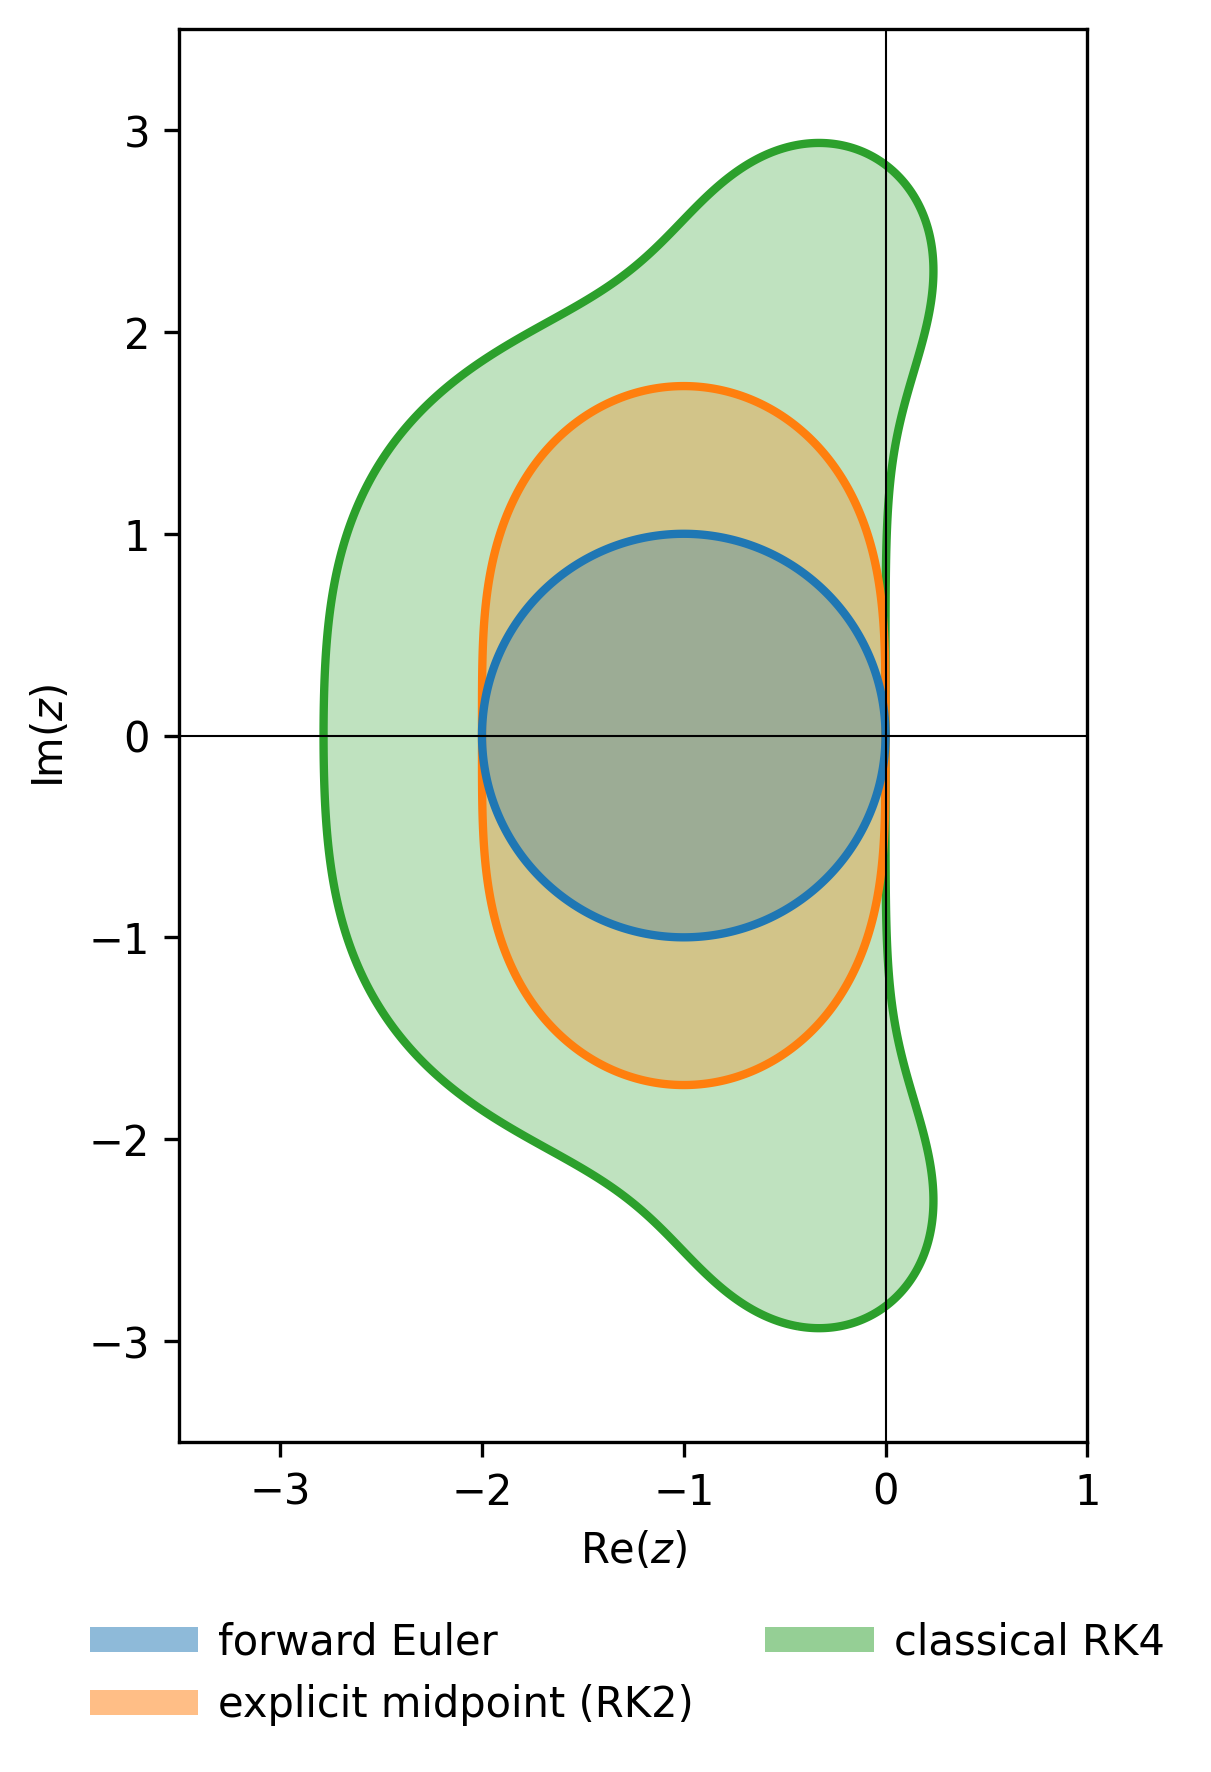
\includegraphics[width=0.6\textwidth]{./Lectures/Lec9/stability_regions_rk.png}
   \caption{Stability regions for various explicit Runge-Kutta methods.}
   \label{fig:RK-stability}
\end{figure}

% \begin{equation*}
%     u(t_n) - u(t_{n-1}) = \int_{t_{n-1}}^{t_n} u'(t) \, dt = \int_{t_{n-1}}^{t_n} f(u(t)) \, dt.
% \end{equation*}



% \bibliographystyle{plainnat}
% \bibliography{references}
\chapter{Higher order methods II: Linear Multistep Methods}



\bibliographystyle{plainnat}
\bibliography{references}




\part{ \; Numerical methods for BVPs}

\chapter{Introduction to finite difference methods}

\bibliographystyle{plainnat}
\bibliography{references}
\chapter{Solving Poisson's equation}

\bibliographystyle{plainnat}
\bibliography{references}
\chapter{A first encounter with spectral methods}

\bibliographystyle{plainnat}
\bibliography{references}
\chapter{A first encounter with finite element methods}

\bibliographystyle{plainnat}
\bibliography{references}

\part{ \; Numerical methods for PDEs}


\chapter{Elliptic, parabolic, and hyperbolic PDEs and some motivating examples}

\bibliographystyle{plainnat}
\bibliography{references}
\chapter{Finite difference methods for the Poisson PDE}


\bibliographystyle{plainnat}
\bibliography{references}
\chapter{Solving the variable coefficient Poisson equation in 2D}

\bibliographystyle{plainnat}
\bibliography{references}
\chapter{The method of lines for solving the heat equation}

\bibliographystyle{plainnat}
\bibliography{references}
\chapter{A second encounter with the finite element method}


\bibliographystyle{plainnat}
\bibliography{references}
\chapter{Solving the Convection-Diffusion-Reaction PDEs in 1D}


\bibliographystyle{plainnat}
\bibliography{references}
\chapter{Operator splitting and IMEX methods}

\bibliographystyle{plainnat}
\bibliography{references}
\chapter{Solving the transport problem and issues with time stepping}

\bibliographystyle{plainnat}
\bibliography{references}
\chapter{Going back to stability and accuracy}


\bibliographystyle{plainnat}
\bibliography{references}
\chapter{Solving the wave equation in 1D}


\bibliographystyle{plainnat}
\bibliography{references}
\chapter{Advanced topic: geometry, mesh generation, and the advantages of finite element methods}

\bibliographystyle{plainnat}
\bibliography{references}
\chapter{Advanced topic: fast convergence and the advantages of spectral methods}

\bibliographystyle{plainnat}
\bibliography{references}
\chapter{Advanced topic: the finite volume method}


\bibliographystyle{plainnat}
\bibliography{references}
\chapter{Advanced topic: physics informed neural networks (PINNs) and deep learning for PDEs}

\bibliographystyle{plainnat}
\bibliography{references}







\part{ \; Review materials}

\appendix

\chapter{Review of applied linear algebra}

The following is a brief review of some basic concepts in linear algebra that will be used throughout the course. Many definitions and results are stated 
without proof. The reader is encouraged to consult standard references 
such as \cite{olver2006applied,boyd2018introduction,demmel1997applied,matrixcookbook}.


\section{Vectors, inner products, and bases}

Write $\R^d$ to denote the $d$-dimensional Euclidean space. 
We will use boldface letter to denote vectors in $\R^d$,
for example $\xb \in \R^d$ to denote the vector 
$\xb = (x_1, x_2, \ldots, x_d)$ with $x_j \in \R$ for $j=1,2,\ldots,d$
denoting the individual entries. The usual Euclidean i`nner product of 
two vectors $\xb, \yb \in \R^d$ is defined as
\begin{equation}\label{def:euclidean-inner-product}
\langle \xb, \yb \rangle := \sum_{j=1}^d x_j y_j.    
\end{equation}

\begin{definition}[Inner product]
    Any function $\iota: \R^d \times \R^d \to \R$ that satisfies 
    the following four axioms is called an inner product on $\R^d$:
    \begin{itemize}
        \item Symmetry: $\iota(\xb, \yb) = \iota(\yb, \xb)$ for all $\xb, \yb \in \R^d$
        \item Linearity: $\iota(\alpha \xb + \beta \yb, \zb) = \alpha \iota(\xb, \zb) + \beta \iota(\yb, \zb)$ for all $\xb, \yb, \zb \in \R^d$ and $\alpha, \beta \in \R$
        \item Positivity: $\iota(\xb, \xb) \ge 0$ for all $\xb \in \R^d$
        \item Definiteness: $\iota(\xb, \xb) = 0$ if and only if $\xb = 0$
    \end{itemize}
\end{definition}
The Euclidean inner product defined in  \eqref{def:euclidean-inner-product}
is indeed an inner product on $\R^d$ according to the above definition.
The proof is straightforward and is left as an exercise for the reader.
We use the bracket notation to distinguish this inner product from 
other inner products that we may encounter later.


\begin{definition}[Norm]
    We say that a function $\|\cdot\|: \R^d \to \R$ is a norm on $\R^d$ if it satisfies the following three axioms:
    \begin{itemize}
        \item Positivity: $\|\xb\| \ge 0$ for all $\xb \in \R^d$
        \item Definiteness: $\|\xb\| = 0$ if and only if $\xb = 0$
        \item Triangle inequality: $\|\xb + \yb\| \le \|\xb\| + \|\yb\|$ for all $\xb, \yb \in \R^d$
    \end{itemize}
\end{definition}
The Euclidean inner product induces the Euclidean norm on $\R^d$, 
also routinely called the $2$-norm or the $\ell^2$-norm, defined as
\begin{equation*}
    \|\xb\|_2 = \sqrt{\langle \xb, \xb \rangle} = \sqrt{\sum_{j=1}^d x_j^2}.
\end{equation*}

With the above notion of inner product and norm, we can define the angle between two vectors and the notion of orthogonality.
The angle between two vectors $\xb$ and $\yb$ is defined as
\begin{equation*}
   \theta(\xb, \yb) \equiv \theta := \arccos \left( \frac{\langle \xb, \yb \rangle}{\|\xb\|_2 \|\yb\|_2} \right),
\end{equation*}
Hence, we say $\xb$ and $\yb$ are orthogonal (with respect to 
the Euclidean inner product) if $\langle \xb, \yb \rangle = 0$,
since it implies that $\theta = \pi/2$.

We say that a set of vectors $\{\xb_1, \xb_2, \ldots, \xb_N\} \equiv 
\{ \xb_j \}_{j=1}^N \subset \R^d$ 
are {\it linearly independent} if the only solution to the equation
\begin{equation*}
    \sum_{j=1}^N \alpha_j \xb_j = 0,
\end{equation*}
is $\alpha_j = 0$ for all $j=1,2,\ldots,N$ otherwise we 
say that they are {\it linearly dependent}.
For a set of vectors $\{\xb_j\}_{j=1}^N$, we also define their {\it span} as
\begin{equation*}
    \Span\{\xb_j\}_{j=1}^N := \left\{ \sum_{j=1}^N \alpha_j \xb_j : \alpha_j \in \R, j=1,2,\ldots,N \right\} \subseteq \R^d.
\end{equation*}
For a subspace $V \subseteq \R^d$, we say that a set of vectors
$\{\xb_j\}_{j=1}^N$ span $V$ if $\Span\{\xb_j\}_{j=1}^N = V$.
We say that a set of vectors $\{\xb_j\}_{j=1}^N$ are a {\it basis} 
for $V$ if they are linearly independent and they span $V$. Bases are 
not necessarily unique, i.e., we can find two sets of linearly 
independent vectors that span the same subspace $V$. However,
the number of vectors in any basis for a subspace $V$ is unique and is called the {\it dimension} of $V$.
\begin{lemma}
    Every subspace $V \subseteq \R^d$ has a basis and any two bases for $V$ have the same number of elements. The number of elements in a basis for $V$ is called the dimension of $V$ and is denoted by $\dim(V)$.
\end{lemma}
Bases are also useful for representing elements of a subspace.

\begin{lemma}
If $\{ \xb_j\}_{j=1}^N$ form a basis for a subspace $V$ then every element 
$\vb \in V$ can be uniquely expressed as a linear combination of 
the $\xb_j$'s, i.e., there exist unique coefficients $\alpha_j \in \R$ such that
$\vb = \sum_{j=1}^N \alpha_j \xb_j.$    
\end{lemma}




We say  $\{\xb_j\}_{j=1}^N$ 
are {\it orthogonal} if $\langle \xb_i, \xb_j \rangle = 0$ for all $i \neq j$.
We further say they are {\it orthonormal} if they are orthogonal and $\|\xb_j\|_2 = 1$ for all $j=1,2,\ldots,N$. 

\begin{lemma}
    Every orthogonal set of non-zero vectors is linearly independent.
\end{lemma}

Given a linearly independent set of vectors $\{ \xb_j \}_{j=1}^N$, 
we can always construct an orthonormal set of vectors $\{\qb_j\}_{j=1}^N$
such that 
\begin{equation*}
    \Span\{\qb_j\}_{j=1}^N = \Span\{\xb_j\}_{j=1}^N.
\end{equation*}
The classic procedure for doing so is called the Gram-Schmidt process: 
\begin{algorithm}
\caption{Gram-Schmidt Process}
\begin{algorithmic}
    \State {\bf Input}: linearly independent set of vectors 
    $\{\xb_j\}_{j=1}^N \subseteq \R^d$.
    \State {\bf Output}: orthonormal set of vectors $\{\qb_j\}_{j=1}^N \subset \R^d$
    \vspace{2ex}
    \State Set $\qb_1 = \xb_1 / \|\xb_1\|_2$.
    \For{$j=2,3,\ldots,N$}
        \State 
        \begin{equation*}
            \qb_j = \frac{\xb_j - \sum_{i=1}^{j-1} \langle \xb_j, \qb_i \rangle \qb_i}{\left\| \xb_j - \sum_{i=1}^{j-1} \langle \xb_j, \qb_i \rangle \qb_i \right\|_2}.
        \end{equation*}
    \EndFor
\end{algorithmic}
\end{algorithm}


\section{Matrices}

For positive integers $m, n$ consider a function $f: \R^n \to \R^m$. 

\begin{definition}[Linear and affine functions]
We say $f: \R^n \to \R^m$ is linear if it satisfies the following two properties:
\begin{itemize}
    \item Additivity: $f(\xb + \yb) = f(\xb) + f(\yb)$ for all $\xb, \yb \in \R^n$
    \item Homogeneity: $f(\alpha \xb) = \alpha f(\xb)$ for all $\xb \in \R^n$ and $\alpha \in \R$
\end{itemize}
We say $g: \R^n \to \R^m$ is affine if there exists a linear function $f: \R^n \to \R^m$ and a vector $\vb \in \R^m$ such that $g(\xb) = f(\xb) + \vb$ for all $\xb \in \R^n$.
\end{definition}

Linear functions from $\R^n$ to $\R$ can be represented as matrix-vector products. More precisely, 
\begin{lemma}
Every linear function $f: \R^n \to \R$ is uniquely associated with 
   with a vector $\fb \in \R^n$ such that $f(\xb) = \langle \fb, \xb \rangle$ for all $\xb \in \R^n$. 
\end{lemma}
In other words, linear functions from $\R^n$ to $\R$ can be identified with (are isomorphic to) vectors in $\R^n$. Additionally, for $f: \R^n \to \R^m$ write $f(\xb) = (f_1(\xb), f_2(\xb), \ldots, f_m(\xb))$ where $f_j: \R^n \to \R$ for $j=1,2,\ldots,m$. Then $f$ is linear if and only if each $f_j$ is linear. Hence, we can represent a linear function $f: \R^n \to \R^m$ 
\begin{equation*}
    f(\xb) = \begin{bmatrix}
        f_1(\xb) \\
        f_2(\xb) \\
        \vdots \\
        f_m(\xb)
    \end{bmatrix} = 
    \begin{bmatrix}
        \langle \fb_1, \xb \rangle \\
        \langle \fb_2, \xb \rangle \\
        \vdots \\
        \langle \fb_m, \xb \rangle
    \end{bmatrix} 
\end{equation*}
Collecting the vectors $\fb_j$ into a list, as the rows of a table, we obtain 
the classic definition of a matrix $F$. 
\begin{definition}
    An $m \times n$ matrix $F$ is a rectangular array of real numbers with $m$ rows and $n$ columns. The entries in the $i$-th row and $j$-th column of $F$ are denoted by $f_{ij}$. The set of all matrices with $m$ rows and $n$ columns is denoted by $\R^{m \times n}$.
\end{definition}

Simply put, given a matrix $F \in \R^{m \times n}$, we think of  
\begin{equation*}
    F = \begin{bmatrix}
        f_{11} & f_{12} & \cdots & f_{1n} \\
        f_{21} & f_{22} & \cdots & f_{2n} \\
        \vdots & \vdots & \ddots & \vdots \\
        f_{m1} & f_{m2} & \cdots & f_{mn}
    \end{bmatrix} 
    \equiv 
    \begin{bmatrix}
        -  & \fb_{1:} &  - \\
        -  & \fb_{2:} &  - \\
         & \vdots &  \\
        -  & \fb_{m:} &  -
    \end{bmatrix} 
    \equiv 
    \begin{bmatrix}
        |        & |        &  |  &      | \\
        \fb_{:1} & \fb_{:2} & \cdots & \fb_{:n} \\
                |        & |        &  |  &      |   
    \end{bmatrix}
\end{equation*}
where we also introduced the \texttt{Python}-style notation $\fb_{j:}$ to 
denote the $j$-th row of $F$ and $\fb_{:j}$ to denote the $j$-th column of $F$.
We will also use the standard notation $F_{ij}$ to denote the 
entries of $F$ in the $i$-th row and $j$-th column, i.e., $F_{ij} = f_{ij}$ in the above 
case. We will also use the shorthand notation $F = (f_{ij})$ to denote a matrix $F$ with entries $f_{ij}$ in the $i$-th row and $j$-th column.

With the above notation we can then define the matrix-vector product $F \xb$ as
\begin{equation*}
    F \xb = f(\xb) = \begin{bmatrix}
        \langle \fb_{1:}, \xb \rangle \\
        \langle \fb_{2:}, \xb \rangle \\
        \vdots \\
        \langle \fb_{m:}, \xb \rangle  
    \end{bmatrix} 
    =  
    \sum_{j=1}^n x_j \fb_{:j}.
\end{equation*}
In words, $F \xb$ denotes the evaluation of the underlying linear function $f$ at 
$\xb$ which can be represented in two ways: (1) as a list of inner products of the rows of $F$ with $\xb$ or (2) as a linear combination of the columns of $F$ with coefficients given by the entries of $\xb$.

For two matrices $F \in \R^{m \times n}$ and $G \in \R^{n \times p}$, we can define their product $FG \in \R^{m \times p}$ as the composition of the underlying linear functions, i.e., $FG \xb = f(g(\xb))$ for all $\xb \in \R^p$. In terms of the entries of $F$ and $G$, we have
\begin{equation*}
    (FG)_{ij} = \sum_{k=1}^n f_{ik} g_{kj} = \langle \fb_{i:}, \gb_{:j} \rangle.
\end{equation*}
Given $F \in \R^{m \times n}$, we can also define the transpose of $F$, denoted by $F^\top \in \R^{n \times m}$, as the matrix with entries $(F^\top)_{ij} = f_{ji}$ for all $i=1,2,\ldots,n$ and $j=1,2,\ldots,m$. In other words, the rows of $F$ become the columns of $F^\top$ and vice versa. Equivalently, we can write $F^\top = (f_{ji})$ to denote the transpose of $F$. The transpose $F^\top$ is the unique matrix in $\R^{n \times m}$ such that $\langle F \xb, \yb \rangle = \langle \xb, F^\top \yb \rangle$ for all $\xb \in \R^n$ and $\yb \in \R^m$.

\begin{definition}
    We say that a matrix $F$ is square if it has the same number of rows and columns, i.e., $F \in \R^{n \times n}$ for some $n \in \N$. We say that a square matrix $F$ is 
    symmetric if $F = F^\top$, i.e., $f_{ij} = f_{ji}$ for all $i,j=1,2,\ldots,n$.
\end{definition}

\begin{definition}
    A square matrix $F \in \R^{n \times n}$ is invertible if there exists a square matrix $G \in \R^{n \times n}$ such that $FG = GF = I_n$ where $I_n$ is the $n \times n$ identity matrix. The matrix $G$ is called the inverse of $F$ and is denoted by $F^{-1}$.
\end{definition}

\begin{lemma}
    Consider $F \in \R^{n \times n}$. Then the following statements are equivalent:

    \begin{itemize}
        \item $F$ is invertible.
        \item The columns of $F$ are linearly independent.
        \item The rows of $F$ are linearly independent.
        \item The equation $F \xb = \yb$ has a unique solution for every $\yb \in \R^n$.
        \item The equation $F \xb = 0$ has only the trivial solution $\xb = 0$.
    \end{itemize}
\end{lemma}

\begin{definition}
    We say that a square matrix $F \in \R^{n \times n}$ is positive definite if $\langle F \xb, \xb \rangle > 0$ for all $\xb \in \R^n$ with $\xb \neq 0$. We say that $F$ is positive semi-definite if $\langle F \xb, \xb \rangle \ge 0$ for all $\xb \in \R^n$.
\end{definition}

Positive definite matrices are some of the nicest objects in linear algebra. For example, 
they are always invertible and their inverses are also positive definite. Additionally, 
a positive definite matrix $F$ induces an inner product and norm on $\R^n$ defined as $\langle \xb, \yb \rangle_F := \langle F \xb, \yb \rangle$ and $\|\xb\|_F := \sqrt{\langle F \xb, \xb \rangle}$ for all $\xb, \yb \in \R^n$.

\section{Extension to complex variables}

All of the ideas and definitions above can be extended to complex variables. We denote the $d$-dimensional complex space by $\C^d$. For $\zb = (z_1, z_2, \ldots, z_d) \in \C^d$ we define its complex conjugate as $\overline{\zb} = (\overline{z_1}, \overline{z_2}, \ldots, \overline{z_d})$ where $\overline{z_j}$ is the complex conjugate of $z_j$ for $j=1,2,\ldots,d$. The Euclidean inner product on $\C^d$ is then defined as 
\begin{equation*}
    \langle \zb, \wb \rangle := \sum_{j=1}^d z_j \overline{w_j} = \langle \overline{\wb}, \overline{\zb} \rangle
\end{equation*}
The notions of norm, orthogonality, linear independence, span, basis, and dimension can be defined in the same way as in the real case. The Gram-Schmidt process can also be applied to complex vectors to obtain an orthonormal set of vectors just as before simply by 
changing our definition of the inner product to the complex inner product defined above.

We can also define complex matrices as before and denote their space as $\C^{n \times m}$. The transpose of a complex matrix $F \in \C^{n \times m}$ is defined as before and is denoted by $F^\top \in \C^{m \times n}$. Additionally, we can define the conjugate transpose of $F$, denoted by $F^* \in \C^{m \times n}$, as the matrix with entries $(F^*)_{ij} = \overline{f_{ji}}$ for all $i=1,2,\ldots,m$ and $j=1,2,\ldots,n$. In other words, the conjugate transpose of a complex matrix is obtained by taking the transpose and then taking the complex conjugate of each entry. The conjugate transpose is also sometimes called the Hermitian transpose and may be denoted as $F^H$ but we will not use this notation. Note that the conjugate transpose of a matrix 
is, in some sense, the more natural extension of the transpose to complex matrices since it satisfies the property $\langle F \zb, \wb \rangle = \langle \zb, F^* \wb \rangle$ for all $\zb \in \C^n$ and $\wb \in \C^m$.

Regardless, a symmetric complex matrix $F \in \R^{n \times n}$ is defined as a matrix that satisfies $F = F^\top$ and a Hermitian complex matrix $F \in \C^{n \times n}$ is defined as a matrix that satisfies $F = F^*$. A Hermitian matrix is the natural extension of a symmetric matrix to complex matrices. A Hermitian matrix $F$ is positive definite if $\langle F \zb, \zb \rangle > 0$ for all $\zb \in \C^n$ with $\zb \neq 0$ and it is positive semi-definite if $\langle F \zb, \zb \rangle \ge 0$ for all $\zb \in \C^n$.


\section{Some special types of matrices}

Certain matrices with special structure appear so frequently in applications and numerical computations that they deserve their own names. We collect a few of the most important ones here.

\begin{definition}[Identity matrix]
    The identity matrix $I_n \in \R^{n \times n}$ is defined entrywise by
    \begin{equation*}
        (I_n)_{ij} = \begin{cases} 1 & i = j \\ 0 & i \neq j \end{cases}, \qquad i,j = 1,2,\ldots,n.
    \end{equation*}
\end{definition}
For example,
\begin{equation*}
    I_3 = \begin{bmatrix}
        1 & 0 & 0 \\
        0 & 1 & 0 \\
        0 & 0 & 1
    \end{bmatrix}.
\end{equation*}
As the name suggests, $I_n$ is the multiplicative identity for matrix multiplication: $I_n F = F I_n = F$ for every $F \in \R^{n \times n}$, and $I_n \xb = \xb$ for every $\xb \in \R^n$. We already used $I_n$ in this way when defining the inverse of a matrix above.

\begin{definition}[Diagonal matrix]
    A square matrix $D \in \R^{n \times n}$ is called diagonal if $(D)_{ij} = 0$ whenever $i \neq j$. We write $D = \mathrm{diag}(d_1, d_2, \ldots, d_n)$ where $d_i = (D)_{ii}$ for $i=1,2,\ldots,n$.
\end{definition}
For example,
\begin{equation*}
    D = \begin{bmatrix}
        2 & 0 & 0 \\
        0 & -1 & 0 \\
        0 & 0 & 5
    \end{bmatrix} = \mathrm{diag}(2,-1,5).
\end{equation*}
The identity matrix is the special case $I_n = \mathrm{diag}(1,1,\ldots,1)$. Diagonal matrices act on vectors by simple entrywise scaling, $(D\xb)_i = d_i x_i$, and the product of two diagonal matrices is again diagonal, obtained by multiplying corresponding diagonal entries. A diagonal matrix $D$ is invertible if and only if $d_i \neq 0$ for every $i$, in which case $D^{-1} = \mathrm{diag}(1/d_1, 1/d_2, \ldots, 1/d_n)$.

\begin{definition}[Triangular matrices]
    A square matrix $U \in \R^{n \times n}$ is called upper triangular if $(U)_{ij} = 0$ whenever $i > j$, and a square matrix $L \in \R^{n \times n}$ is called lower triangular if $(L)_{ij} = 0$ whenever $i < j$.
\end{definition}
For example,
\begin{equation*}
    U = \begin{bmatrix}
        1 & 2 & 3 \\
        0 & 4 & 5 \\
        0 & 0 & 6
    \end{bmatrix}, \qquad
    L = \begin{bmatrix}
        1 & 0 & 0 \\
        2 & 4 & 0 \\
        3 & 5 & 6
    \end{bmatrix}
\end{equation*}
are, respectively, upper and lower triangular. Note that $L = U^\top$ in this example; in general the transpose of an upper triangular matrix is lower triangular and vice versa. Diagonal matrices are simultaneously upper and lower triangular. The sum or product of two upper (lower) triangular matrices is again upper (lower) triangular, and a triangular matrix is invertible if and only if all of its diagonal entries are nonzero, in which case its inverse is triangular of the same type. Triangular matrices are important because linear systems $U\xb = \yb$ or $L\xb = \yb$ can be solved efficiently by back- or forward-substitution; this is the basis of the $LU$ decomposition discussed below.

\begin{definition}[Orthogonal matrix]
    A square matrix $Q \in \R^{n \times n}$ is called orthogonal if
    \begin{equation*}
        Q^\top Q = Q Q^\top = I_n,
    \end{equation*}
    or equivalently $Q^{-1} = Q^\top$.
\end{definition}
Equivalently, $Q$ is orthogonal precisely when its columns (or, equivalently, its rows) form an orthonormal set of vectors in $\R^n$ with respect to the Euclidean inner product \eqref{def:euclidean-inner-product}. A useful consequence is that orthogonal matrices preserve inner products and norms:
\begin{equation*}
    \langle Q\xb, Q\yb \rangle = \langle \xb, \yb \rangle, \qquad \|Q\xb\|_2 = \|\xb\|_2, \qquad \text{for all } \xb, \yb \in \R^n.
\end{equation*}
For example, the permutation matrix
\begin{equation*}
    Q_1 = \begin{bmatrix}
        0 & 1 & 0 \\
        0 & 0 & 1 \\
        1 & 0 & 0
    \end{bmatrix}
\end{equation*}
is orthogonal since its columns are just the standard basis vectors of $\R^3$ in a different order. Another example is the rotation matrix
\begin{equation*}
    Q_2 = \begin{bmatrix}
        \cos\theta & -\sin\theta & 0 \\
        \sin\theta & \cos\theta & 0 \\
        0 & 0 & 1
    \end{bmatrix},
\end{equation*}
which rotates $\R^3$ by an angle $\theta$ about the third coordinate axis; one can check directly that $Q_2^\top Q_2 = I_3$ for any choice of $\theta$.

\begin{definition}[Unitary matrix]
    A square matrix $U \in \C^{n \times n}$ is called unitary if
    \begin{equation*}
        U^* U = U U^* = I_n,
    \end{equation*}
    or equivalently $U^{-1} = U^*$.
\end{definition}
As with the orthogonal case, $U$ is unitary precisely when its columns (or rows) form an orthonormal set of vectors in $\C^n$ with respect to the complex inner product introduced above, and unitary matrices preserve the complex inner product and norm in the same way that orthogonal matrices do on $\R^n$. In fact, orthogonal matrices are exactly the real unitary matrices: when all entries of $U$ are real, the conjugate transpose $U^*$ coincides with the transpose $U^\top$. A simple example of a unitary matrix is a diagonal matrix whose entries have unit modulus, such as
\begin{equation*}
    U_1 = \begin{bmatrix}
        1 & 0 & 0 \\
        0 & i & 0 \\
        0 & 0 & -1
    \end{bmatrix},
\end{equation*}
since $U_1^* U_1 = \mathrm{diag}(|1|^2, |i|^2, |-1|^2) = I_3$. A less trivial example, which will reappear later in the course in connection with the discrete Fourier transform, is
\begin{equation*}
    U_2 = \frac{1}{\sqrt{3}}\begin{bmatrix}
        1 & 1 & 1 \\
        1 & \omega & \omega^2 \\
        1 & \omega^2 & \omega
    \end{bmatrix}, \qquad \omega = e^{2\pi i/3},
\end{equation*}
whose columns can be checked to be orthonormal with respect to the complex inner product.

\section{Useful matrix decompositions}

A matrix decomposition rewrites a matrix as a product of matrices with simpler structure, such as the special types introduced above. Decompositions are central to numerical linear algebra: they are the standard tools for solving linear systems, least-squares problems, and eigenvalue problems efficiently and stably. We simply state the definitions here; the algorithms used to compute these decompositions can be 
found in classic references such as \cite{demmel1997applied,olver2006applied}.

\begin{definition}[LU decomposition]
    Let $F \in \R^{n \times n}$ be a matrix that can be reduced to upper triangular form using only row operations that add a multiple of one row to another (i.e., without row interchanges). Then there exist a unit lower triangular matrix $L \in \R^{n \times n}$ (i.e., lower triangular with $(L)_{ii}=1$ for all $i$) and an upper triangular matrix $U \in \R^{n \times n}$ such that
    \begin{equation*}
        F = LU.
    \end{equation*}
\end{definition}
The entries of $L$ record the multipliers used during Gaussian elimination, and $U$ is the resulting upper triangular matrix. Once $F$ has been factored in this way, the linear system $F\xb = \yb$ reduces to two easy triangular solves: $L\zb = \yb$ followed by $U\xb = \zb$. For example,
\begin{equation*}
    F = \begin{bmatrix}
        2 & 1 & 1 \\
        4 & 3 & 3 \\
        8 & 7 & 9
    \end{bmatrix}
    =
    \underbrace{\begin{bmatrix}
        1 & 0 & 0 \\
        2 & 1 & 0 \\
        4 & 3 & 1
    \end{bmatrix}}_{L}
    \underbrace{\begin{bmatrix}
        2 & 1 & 1 \\
        0 & 1 & 1 \\
        0 & 0 & 2
    \end{bmatrix}}_{U}.
\end{equation*}

\begin{definition}[QR decomposition]
    Let $F \in \R^{n \times n}$ be invertible. Then there exist an orthogonal matrix $Q \in \R^{n \times n}$ and an upper triangular matrix $R \in \R^{n \times n}$ with positive diagonal entries such that
    \begin{equation*}
        F = QR.
    \end{equation*}
\end{definition}
This decomposition is precisely what results from applying the Gram-Schmidt process to the columns of $F$: the columns of $Q$ are the resulting orthonormal vectors, and the entries of $R$ record the coefficients used in forming each column of $F$ as a linear combination of the columns of $Q$. For example,
\begin{equation*}
    F = \begin{bmatrix}
        12 & -51 & 4 \\
        6 & 167 & -68 \\
        -4 & 24 & -41
    \end{bmatrix}
    =
    \underbrace{\frac{1}{175}\begin{bmatrix}
        150 & -69 & -58 \\
        75 & 158 & 6 \\
        -50 & 30 & -165
    \end{bmatrix}}_{Q}
    \underbrace{\begin{bmatrix}
        14 & 21 & -14 \\
        0 & 175 & -70 \\
        0 & 0 & 35
    \end{bmatrix}}_{R}.
\end{equation*}

\begin{definition}[Cholesky decomposition]
    Let $F \in \R^{n \times n}$ be symmetric positive definite. Then there exists a unique lower triangular matrix $L \in \R^{n \times n}$ with positive diagonal entries such that
    \begin{equation*}
        F = LL^\top.
    \end{equation*}
\end{definition}
The Cholesky decomposition can be viewed as a kind of matrix square root for positive definite matrices, and also as a symmetric special case of the $LU$ decomposition in which $U = L^\top$. For example,
\begin{equation*}
    F = \begin{bmatrix}
        4 & 12 & -16 \\
        12 & 37 & -43 \\
        -16 & -43 & 98
    \end{bmatrix}
    =
    \underbrace{\begin{bmatrix}
        2 & 0 & 0 \\
        6 & 1 & 0 \\
        -8 & 5 & 3
    \end{bmatrix}}_{L}
    \underbrace{\begin{bmatrix}
        2 & 6 & -8 \\
        0 & 1 & 5 \\
        0 & 0 & 3
    \end{bmatrix}}_{L^\top}.
\end{equation*}

\begin{definition}[Singular value decomposition]
    Let $F \in \R^{m \times n}$ be any matrix (not necessarily square). Then there exist orthogonal matrices $U \in \R^{m \times m}$ and $V \in \R^{n \times n}$, and a matrix $\Sigma \in \R^{m \times n}$ that is zero off of its main diagonal with nonnegative diagonal entries $\sigma_1 \ge \sigma_2 \ge \cdots \ge 0$, such that
    \begin{equation*}
        F = U \Sigma V^\top.
    \end{equation*}
    The $\sigma_j$ are called the singular values of $F$, and the columns of $U$ and $V$ are called, respectively, the left and right singular vectors of $F$.
\end{definition}
Unlike the previous three decompositions, the SVD exists for \emph{every} matrix $F$, regardless of its shape or rank, which makes it one of the most versatile tools in numerical linear algebra. For example,
\begin{equation*}
    F = \begin{bmatrix}
        4 & 1 & 6 \\
        -2 & -2 & 6 \\
        -4 & 2 & 3
    \end{bmatrix}
    =
    \underbrace{\frac{1}{3}\begin{bmatrix}
        2 & 2 & 1 \\
        2 & -1 & -2 \\
        1 & -2 & 2
    \end{bmatrix}}_{U}
    \underbrace{\begin{bmatrix}
        9 & 0 & 0 \\
        0 & 6 & 0 \\
        0 & 0 & 3
    \end{bmatrix}}_{\Sigma}
    \underbrace{\begin{bmatrix}
        0 & 0 & 1 \\
        1 & 0 & 0 \\
        0 & 1 & 0
    \end{bmatrix}}_{V^\top}.
\end{equation*}


\section{Eigenvalue decompositions}

Throughout this course we will heavily rely on the eigenvalue decomposition of 
a matrix to make sense of many ideas from stability and convergence 
properties of ODEs and numerical algorithms to the design of 
efficient algorithms such as spectral methods. 

\begin{definition}
    Consider $F \in \C^{n \times n}$. A nonzero vector $\qb \in \C^n$ is called an eigenvector of $F$ if there exists a scalar $\lambda \in \C$ such that
    \begin{equation*}
        F \qb = \lambda \qb.
    \end{equation*}
    We call $(\lambda, \qb)$ an eigenpair of $F$.
\end{definition}
We say that $F$ is diagonalizable if it has $n$ 
linearly independent eigenvectors. In that case, we obtain an eigenvalue 
decomposition (eigen-decomposition for short) of $F$ as
\begin{equation*}
    F = Q \Lambda Q^{-1}
\end{equation*}
where $Q \in \C^{n \times n}$ is the matrix whose columns are
the eigenvectors of $F$ and $\Lambda \in \C^{n \times n}$ is the diagonal matrix whose diagonal entries are the corresponding eigenvalues of $F$.

It is important to note that not every matrix is diagonalizable 
and the eigendecomposition does not exist like the SVD.

\begin{example}
    The following matrix is not diagonalizable:
    \begin{equation*}
        F 
= \begin{bmatrix}
            1 & 1 \\
            0 & 1
        \end{bmatrix}
    \end{equation*}
To see this try to compute the eigenvalues of $F$ by solving the characteristic polynomial $\det(F - \lambda I) = 0$. We have
\begin{equation*}
    \det(F - \lambda I) = \det\begin{bmatrix}
        1 - \lambda & 1 \\
        0 & 1 - \lambda
    \end{bmatrix} = (1 - \lambda)^2.
\end{equation*}
Hence, the only eigenvalue of $F$ is $\lambda = 1$. To find the corresponding eigenvectors we solve the equation $(F - I)\qb = 0$ which gives
\begin{equation*}
    \begin{bmatrix}
        0 & 1 \\
        0 & 0
    \end{bmatrix} \begin{bmatrix}
        q_1 \\
        q_2
    \end{bmatrix} = \begin{bmatrix}
        0 \\
        0
    \end{bmatrix}.
\end{equation*}
This gives the equation $q_2 = 0$ and hence the eigenvectors of $F$ are of the form $\qb = (q_1, 0)^\top$. In particular, there is only one linearly independent eigenvector of $F$ and hence $F$ is not diagonalizable.
\end{example}

\begin{lemma}
    Suppose $F \in \C^{n \times n}$ is Hermitian. 
    Then $F$ is diagonalizable and all of its eigenvalues are real, i.e., 
    there exists a unitary matrix $Q \in \C^{n \times n}$ and a diagonal matrix $\Lambda \in \R^{n \times n}$ such that
    \begin{equation*}
        F = Q \Lambda Q^*.
    \end{equation*}
    If $F$ is also positive semi-definite, then all of its eigenvalues are nonnegative. If $F$ is positive definite, then all of its eigenvalues are positive.
\end{lemma}

\begin{example}
    Consider the matrix 
    \begin{equation*}
        F = \begin{bmatrix}
            1 & - i & 0 \\ 
            i & 1 & -i \\ 
            0 & i & 1
        \end{bmatrix}
    \end{equation*}
    It is easy to check that $F$ is Hermitian since $F^* = F$. Then it has an eigen-decomposition $F = Q \Lambda Q^*$ where
    \begin{equation*}
        Q =  \begin{bmatrix}
            \frac12 & \frac{1}{\sqrt{2}} & \frac12 \\
            -\frac{i}{\sqrt{2}} & 0 & \frac{i}{\sqrt{2}} \\
            - \frac12 & \frac{1}{\sqrt{2}} & -\frac12
        \end{bmatrix}, \qquad
        \Lambda = \begin{bmatrix}
            1 - \sqrt{2} & 0 & 0 \\
            0 & 1 & 0 \\
            0 & 0 & 1 + \sqrt{2}
        \end{bmatrix}.
    \end{equation*}
\end{example}


\section{Matrix powers and exponential}
For a square matrix $F \in \C^{n \times n}$ we can define its powers $F^k$ for $k \in \N$ as the product of $k$ copies of $F$, i.e., $F^k = F F \cdots F$ ($k$ times). We also define $F^0 = I_n$. If $F$ is diagonalizable with eigen-decomposition $F = Q \Lambda Q^{-1}$, then we can compute its powers as
\begin{equation*}
    F^k = Q \Lambda^k Q^{-1}
\end{equation*}
where $\Lambda^k$ is the diagonal matrix with entries $(\Lambda^k)_{ii} = \lambda_i^k$ for $i=1,2,\ldots,n$. This is a very useful property since it allows us to compute powers of $F$ by simply raising its eigenvalues to the $k$-th power.

With matrix powers at hand, we can define polynomial functions of 
matrices $p(F)$ for a polynomial $p(x) = \sum_{k=0}^m a_k x^k$ as
\begin{equation*}
    p(F) = \sum_{k=0}^m a_k F^k.
\end{equation*}
 If $F$ is diagonalizable this takes the form
\begin{equation*}
p(F) = Q p(\Lambda) Q^{-1}
\end{equation*}
where $p(\Lambda)$ is the diagonal matrix with entries $(p(\Lambda))_{ii} = p(\lambda_i)$ for $i=1,2,\ldots,n$. 

Finally, using the Taylor series expansion of the exponential function, we can define the matrix exponential as
\begin{equation*}
    e^F = \sum_{k=0}^\infty \frac{F^k}{k!},
\end{equation*}
which for a diagonalizable matrix $F$ takes the simpler form 
\begin{equation*}
    e^F = Q e^{\Lambda} Q^{-1}.
\end{equation*}

\section{Kronecker products}

The Kronecker product of two matrices $A \in \C^{m \times n}$ and $B \in \C^{p \times q}$ is defined as the block matrix
\begin{equation*}
    A \otimes B = \begin{bmatrix}
        a_{11} B & a_{12} B & \cdots & a_{1n} B \\
        a_{21} B & a_{22} B & \cdots & a_{2n} B \\
        \vdots & \vdots & \ddots & \vdots \\
        a_{m1} B & a_{m2} B & \cdots & a_{mn} B
    \end{bmatrix} \in \C^{mp \times nq}.
\end{equation*}
Some important properties of the Kronecker product include:
\begin{itemize}
    \item $(A \otimes B)(C \otimes D) = (AC) \otimes (BD)$, provided the matrix multiplications $AC$ and $BD$ are defined.
    \item $(A \otimes B)^* = A^* \otimes B^*$.
    \item If $A$ and $B$ are invertible, then $(A \otimes B)^{-1} = A^{-1} \otimes B^{-1}$.
    \item If $A$ and $B$ are diagonalizable with $A = Q_A \Lambda_A Q_A^{-1}$ and $B = Q_B \Lambda_B Q_B^{-1}$, then
    \begin{equation*}
        A \otimes B = (Q_A \otimes Q_B)(\Lambda_A \otimes \Lambda_B)(Q_A \otimes Q_B)^{-1}.
    \end{equation*}
\end{itemize}
Perhaps most consequential for us is the property that the Kronecker product interacts nicely with the vectorization of matrices. Specifically, for matrices $A \in \C^{m \times n}$, $B \in \C^{p \times q}$, and $X \in \C^{n \times p}$, we have
\begin{equation}\label{eq:vec-kronecker}
    \text{vec}(AXB) = (B^T \otimes A) \text{vec}(X),
\end{equation}
where $\text{vec}(X)$ denotes the vectorization of $X$ obtained by stacking its columns into a single column vector.


\bibliographystyle{plainnat}
\bibliography{references}






\chapter{Review of calculus}

The following is a brief review of some concepts from 
calculus that we will use throughout the course. 
For a more detailed treatment see the classic texts 
\cite{apostol1991calculus-1,apostol1991calculus-2, babyrudin}.


\section{Partial derivatives, gradients, and other useful operators}

\section{Taylor's theorem}

\section{Integration by parts and Green's identities}

\section{Differentiating functions of vectors and matrices}

\bibliographystyle{plainnat}
\bibliography{references}
\chapter{Review of analytic methods for solving ODEs and PDEs}

\section{Solving ODEs}

\subsection{General and particular solutions}

\subsection{Separation of variables}

\subsection{Integrating factors}
multiple by some exponential so that the left hand side becomes a total derivative


\subsection{Exact solutions}

Potentials etc

\subsection{Substitutions}

Change of variable to reduce to a solvable form

\subsection{Transformations and series}

\begin{itemize}
    \item power series and Frobenius method
    \item Laplace transform
    \item Fourier transform
    \item Fourier series
    \item Green's functions
\end{itemize}

\subsection{Solving systems}

Eigenvalue decomposition, Jordan form, etc



\section{Solving PDEs}

\subsection{Dealing with boundary conditions}

\subsection{Reduction to ODEs}

\begin{itemize}
    \item Separation of variables
    \item Similarity and self-similar solutions 
    \item Eigenfunction expansions
    \item Traveling waves
\end{itemize}

\subsection{Method of characteristics}



\subsection{Transformations}

\begin{itemize}
    \item Fourier
    \item Laplace
    \item Green's functions and fundamental solutions
\end{itemize}




\bibliographystyle{plainnat}
\bibliography{references}

\end{document}